\section{Einrichtung der Ultraschallsensoren}
In diesem Kapitel wird die Verwendung der Ultraschallsensoren in Verbindung mit \acrshort{ros} beschrieben.

\subsection{Erzeugen einer Punktwolke}
Ein Beispiel zur Erzeugung von Punktwolken mit Python ist gegeben unter \footnote{\url{https://docs.ros.org/en/noetic/api/rospy_tutorials/html/publish__pointcloud2_8py_source.html}}, es erzeugt das Bild \ref{fig:ultra_pc_ex}. (Dieses bewegt sich gleichzeitig noch wellenartig.)

Das \acrshort{ros}-Punktwolkenformat definiert eine Klasse mit den Eigenschaften:
\begin{description}
    \item[Header:]
    \begin{itemize}
        \item[]
        \item stamp - aktueller Zeitstempel
        \item frame\_id - Kennzeichnung zur Transformation
    \end{itemize}
    \item[Fields:] Liste von Eigenschaften der Punkte, beihaltet x-,y-,z-Position sowie Farbattribute
    \item[Points:] Liste von Punkten, jeder Punkt im Format wie \enquote{Fields}
\end{description}

Der Zeitstempel wird mit jeder publizierten Nachricht auf die aktuelle Zeit angepasst.

Für die Anwendung im Projekt ist muss die \enquote{frame\_id} eine entsprechende Transformation von der lokalen Position der Drohne besitzen. Im einfachsten Fall wird die Drohne selbst als Ursprungspunkt des Bildes angenommen sodass keine Transformation benötigt wird. Somit entspricht die verwendete \enquote{frame\_id} vorerst immer \enquote{fcu}.

Als Fields kommen die 3 Raumkoordinaten und ein Farbfeld (Achtung hier Abweichung vom Beispiel) zum Einsatz. Das Farbfeld dient der Darstellung in \textit{rviz}, spielt aber für den Einsatzzweck keine Rolle.\\

Zur Erprobung wird eine Liste von Punkten angelegt. Diese befinden sich in 4 Ecken um den Koordinatenursprung (\enquote{fcu}) und einmal direkt darüber. Die Abstände sind jeweils $1m$ in x- und y-Richtung sowie $1m$ in z-Richtung für den z-Punkt. Die Topic der Nachricht wird mit $4Hz$ veröffentlicht, was der Update Rate der Sensoren entspricht \cite[Kapitel 4.4]{markusreinErweiterungBestehenderDrohnen2023}. Das Script ist im Anhang \ref{listing:pcl_test.py} abgedruckt, das Ergebnis zu sehen hier in Bild \ref{fig:ultra_pc_test}. Zur Zeichnung im Bild gibt es noch keine Transformation. Das Koordinatensystem \enquote{fcu} wird daher als Ursprung angenommen (die Einstellung ist oben links in \textit{rviz} zu sehen).

\begin{figure}[!h]
    \centering
    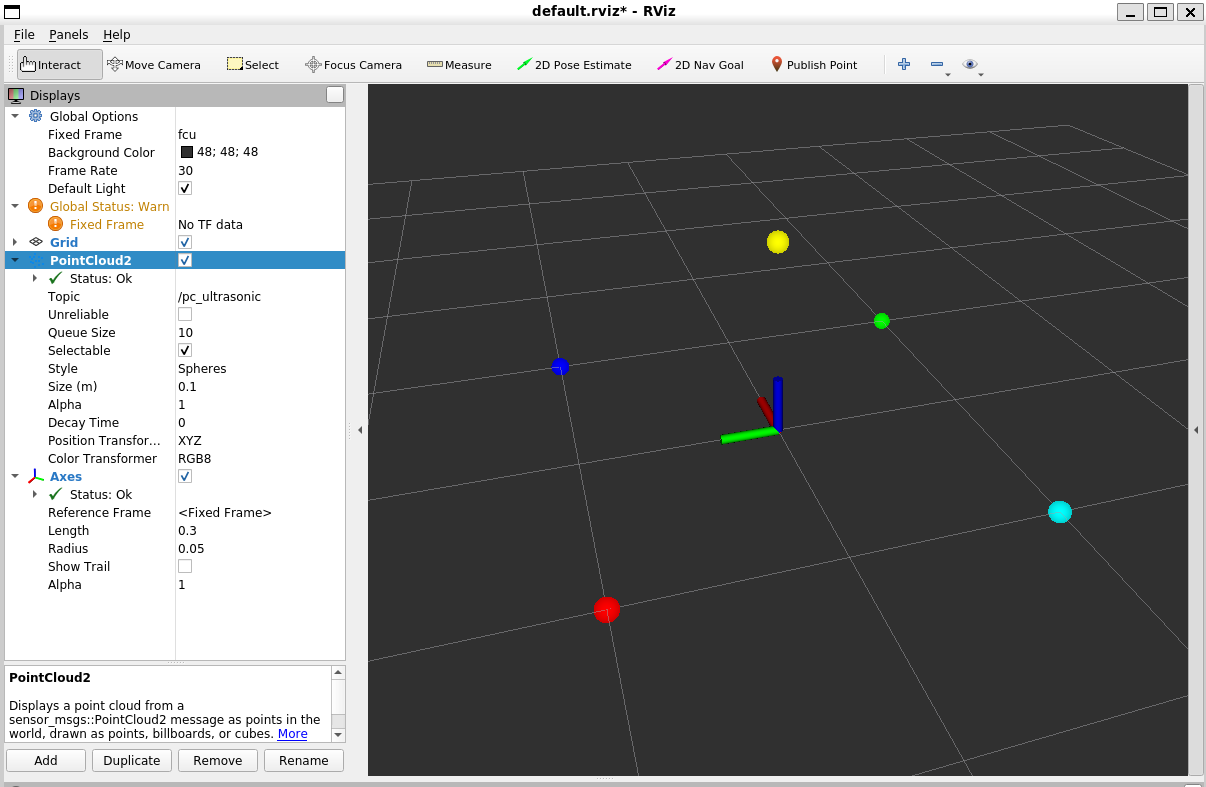
\includegraphics[width=0.7\linewidth]{images/ultra_pc_test.png}
    \caption[Erprobung von Punktwolkenformat]{Erprobung von Punktwolkenformat in \textit{rviz}: die Punkte jeweils im Abstand von $1m$ zum Ursprung. Als Referenz wurde noch ein Koordinatensystem am Ursprung eingezeichnet, bei diesem enspricht x-Achse=rot, y-Achse=grün, z-Achse=blau.}
    \label{fig:ultra_pc_test}
\end{figure}

Zur weiteren Erprobung wird die Simulation gestartet. Die 5 erzeugten Punkte sollten sich gemeinsam mit der Drohne bewegen. In Bild \ref{fig:ultra_pc_test_sim} wurde die Software-Simulation mit Stereokamera gestartet. Anschließend wurde das Script zur Erzeugung von Punktwolken gestartet und in \textit{rviz} hinzugefügt. Zu sehen ist die \enquote{Drohne} (Ursprung der Drohne) mit Punkten, welche sich mitbewegen. Die Bewegung der Punkte ist durch die geringe Update Rate immer etwas später als die der Drohne. Dies sollte aber kein Problem sein, denn es spiegelt das reale Verhalten (die Punkte bleiben stehen aber die Drohne bewegt sich auf diese zu/weg) wieder.

\begin{figure}[!h]
    \centering
    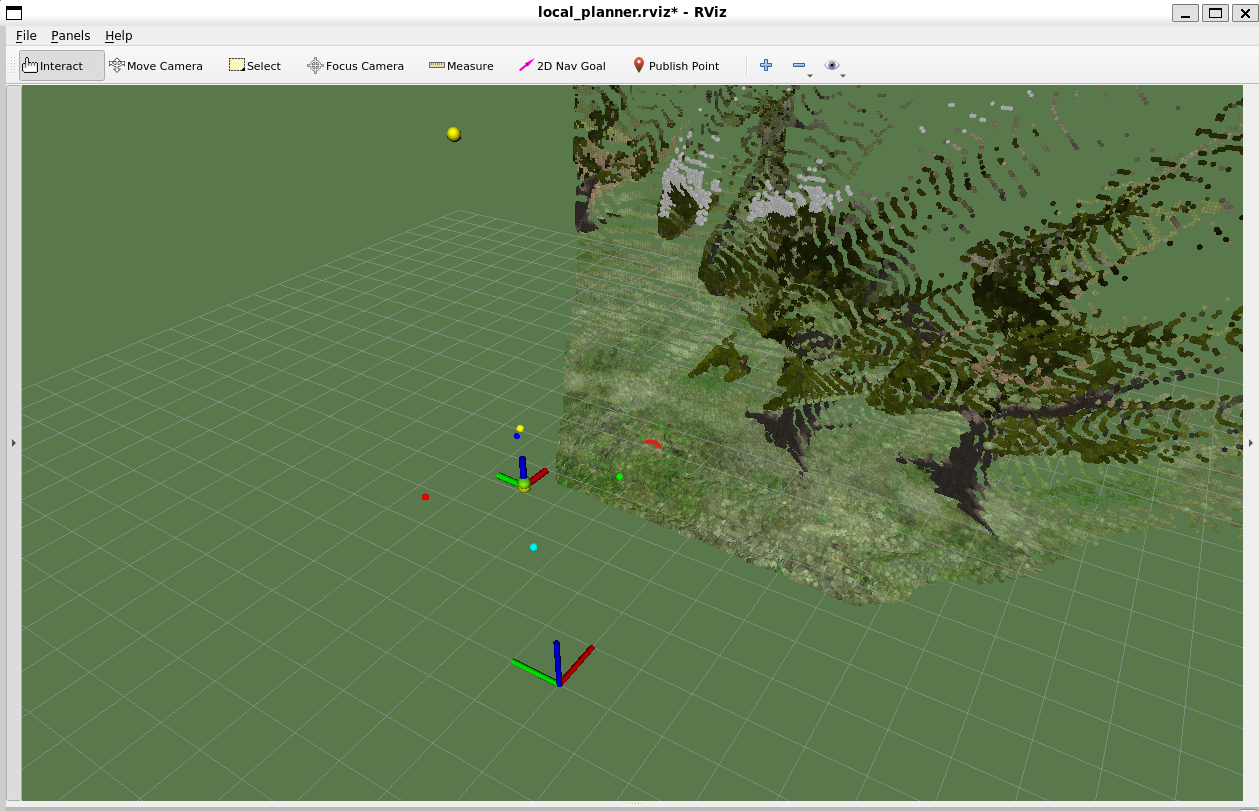
\includegraphics[width=0.7\linewidth]{images/ultra_pc_test_sim.png}
    \caption[Erprobung von Punktwolkenformat mit Simulator]{Erprobung von Punktwolkenformat mit Simulator: die Drohne befindet sich in der Luft vor den Bäumen, um sie herum sind die erzeugten Punkte eingezeichnet.}
    \label{fig:ultra_pc_test_sim}
\end{figure}

\subsection{Software der Sensoren}
Der Algorithmus zum Auslesen der Sensoren wurde bereits für \cite[Kapitel 4.4]{markusreinErweiterungBestehenderDrohnen2023} entworfen, aber die Anwendung noch nicht dokumentiert. Der Code des Projektteils ist auf GitHub unter \footnote{\url{https://github.com/aur20/T3000-autonomous_drone/tree/arduino_sensors}} hinterlegt. Er besteht aus 2 Teilen:

Die \textbf{\large Arduino Firmware} liest die Sensoren aus und stellt Daten per \gls{i2c} zur Verfügung.

Das Auslesen der Sensoren ist mit der notwendigen Verzögerung verbunden, um eventuellen Echos von Ultraschall vorzubeugen. In \ref{listing:ultra_arduino_loop} dargestellt ist ein Ausschnitt aus der loop()-Schleife, die fortwährend immer durchlaufen wird. Der gezeigte Code kommt 4-mal vor, jeweils mit geänderten Pins der Sensoren (Zeile 187) und geänderten Indizes (Zeile 188-190). In der ersten gezeigten Zeile wird der jeweilige Sensor ausgelesen. Dazu wird mittels einer Arduino-internen Funktionen bis zum empfangenen Echo gewartet und die Zeit zurückgegeben. Anschließend wird der gefilterte Sensorwert berechnet. Der ungefilterte und gefilterte Wert werden jeweils in ein Array eingetragen. Zuletzt erfolgt das Warten, mit einer groben Annäherung: das Makro $PAUSE\_MEAS$ steht für $60ms$. Davon abgezogen wird die Zeit, die bereits auf das Echo gewartet wurde in Millisekunden. Arduino selbst stellt eine Verzögerungsfunktion in Mikrosekunden bereit, dieses sollte jedoch nicht für Verzögerungen länger als \enquote{a few thousend microseconds}\footnote{\url{https://www.arduino.cc/reference/en/language/functions/time/delaymicroseconds/}} verwendet werden, und funktioniert auch nur bis zu $16ms$ Verzögerung. Um die Zeit von Mikrosekunden in Millisekunden umzurechnen, muss durch $1000$ geteilt werden. Im Programm wird stattdessen $10$ mal nach rechts geschoben, was einer Division durch $1024$ entspricht. Die Verarbeitung von Schiebeoperationen ist wesentlich schneller als eine Division. Letztere kann im benötigten Zahlenbereich von kleiner $30.000$ zwar mit Integer Variablen umgesetzt werden, benötigt dann aber nach \footnote{\url{https://forum.arduino.cc/t/speed-of-math-operations-particularly-division-on-arduino/90726/5}} immer noch bis zu $15ms$, was die Messfrequenz beeinflussen würde. Außerdem hat der Prozessor bereits Zeit mit der Berechnung des Filters verbracht, sodass die Wartezeit lediglich eine Annäherung an $60ms$ ist, für das Ergebnis spielt dies keine Rolle.  

\begin{listing}[!ht]
    \cccode[firstline=187, lastline=191]{snippets/ultrasonic_arduino.ino}
    \caption{Ausschnitt der Arduino Firmware: loop()-Schleife}
    \label{listing:ultra_arduino_loop}
\end{listing}

Neben dem Auslesen der Sensoren stellt sich der Arduino als \gls{i2c}-Slave zur Verfügung. Er reagiert auf einzelne zugesendete Buchstaben und Zahlen und sendet eine entsprechende Antwort. Derzeit implementiert sind die Funktionen wie in \ref{tab:ultra_arduino_impl_i2c} aufgezeigt.

\begin{table}[!ht]
    \centering
    \caption{Verfügbare Kommandos zum Auslesen der Sensordaten auf Arduino}
    \begin{tabularx}{0.7\textwidth}{ l | l }
    Kommando & Anwort \\ \hline
    eine der Zahlen $1$-$4$ & jeweiliger Sensorwert, gefiltert\\
    Buchstabe \enquote{a} & alle Sensorwerte, gefiltert\\
    Buchstabe \enquote{r} & alle Sensorwerte, ungefiltert
    \label{tab:ultra_arduino_impl_i2c}
    \end{tabularx}
\end{table}

Das \textbf{\large Python Script} auf dem \gls{rpi} gibt Messwerte aus oder speichert diese als \acrshort{csv}-Datei ab.

Derzeit stehen die Scripte \textit{ultrasonic\_i2c\_reader.py} und \textit{ultrasonic\_i2c\_csvwriter.py} zur Verfügung. Sie verhalten sich nahezu gleich. Bei ersterem kann durch die Eingabe eines Zeichens ein bestimmter Wert an den Arduino gesendet werden. Die Antwort wird entsprechend auf der Konsole ausgegeben.\\
Beim zweiten Script kommt nur der Buchstabe \enquote{a} zum Einsatz. Es wird die Antwort geparst und mit aktuellem Zeitstempel in die Datei eingetragen. \ref{listing:ultra_rpi_impl_i2c} zeigt einen Ausschnitt aus der Schleife des zweiten Scriptes. In Zeile 25 werden die Daten per \gls{i2c}-Verbindung gelesen. Um die 16 Byte Binärdaten als Fließkommazahlen zu interpretieren wird das Packet \enquote{struct} verwendet. Im Beispiel werden die Daten in Zeile 28 als Fließkommazahlen im Little-Endian Format interpretiert. Die Funktion \textit{struct.iter\_unpack} liefert anschließend ein iterierbares Objekt (\enquote{Each iteration yields a tuple as specified by the format string.}\footnote{\url{https://docs.python.org/3/library/struct.html}}). Um den Inhalt zu extrahieren wird eine Lambda-Funktion innerhalb der Funktion \textit{map} verwendet, dies hat zur Folge dass jedes Tupel einzeln betrachtet werden kann. Es wird die jeweilige Zahl extrahiert und in einer Liste angelegt. Die Liste wird zusammen mit der derzeitigen Zeit jeweils ausgegeben und in die Datei geschrieben.

\begin{listing}[!ht]
    \pycode[firstline=25, lastline=30]{snippets/ultrasonic_i2c_csvwriter.py}
    \caption{Ausschnitt des Python Scriptes zum Auslesen der Sensordaten}
    \label{listing:ultra_rpi_impl_i2c}
\end{listing}

\subsection{Einbinden der Sensoren}
Als nächster Schritt wurden die vorliegenden Programme miteinander vereinigt.
Vom letzten Script werden jeweils alle 4 Sensoren ausgelesen. Aufgrund der Ungenauigkeit der Messwerte, wurde der Wertebereich nochmals eingeschränkt und beträgt hier $3m$. Größere Werte (beinhaltet Werte außerhalb der Reichweite, die mit $4m$ gesendet werden) werden schlichtweg ignoriert. Die Angaben für die Punktwolke werden auf Meter umgerechnet.

Das Projekt liegt separat auf GitHub\footnote{\url{https://github.com/aur20/T3000-autonomous_drone/tree/rpi_ros_ultrasonic}} und kann innerhalb zukünftiger Container direkt eingebunden werden.

\subsection{Verbesserung der Aufnahmegenauigkeit der Sensoren}
Um die Aufnahmegenauigkeit der Sensoren zu verbessern, könnte eine Interrupt gesteuerte Auslösung des Messvorgangs zum Einsatz kommen. Ein Timer könnte nach jeweils $60ms$ auslösen um die Messung und Berechnungen des Filters durchzuführen.
% Der notwendige Code ist gezeigt in , wurde aber nicht mit der realen Drohne getestet.

